\documentclass[english]{scrartcl}
\usepackage[T1]{fontenc}
\usepackage[utf8]{inputenc}
\usepackage[scaled=.8]{beramono}
\usepackage{geometry}
\geometry{verbose,tmargin=3cm,bmargin=3cm,lmargin=3cm,rmargin=3cm}
\usepackage{microtype}
\usepackage[parfill]{parskip}
\usepackage{amsmath}
\usepackage{graphicx}
\usepackage{hyperref}
\usepackage{nameref}
\usepackage{float}
\usepackage{listings}
\usepackage{color}
\usepackage{fancyhdr}
\usepackage{blindtext}

\pagestyle{fancy}
\fancyhf{}
\rhead{A Team}
\lhead{CC: PaaS}
\cfoot{\thepage}

\newcommand*{\fullref}[1]{\hyperref[{#1}]{\autoref*{#1}~\nameref*{#1}}}

\definecolor{darkgray}{rgb}{0.66, 0.66, 0.66}
\definecolor{asparagus}{rgb}{0.53, 0.66, 0.42}

\lstdefinestyle{s}{
  commentstyle=\color{darkgray},
  keywordstyle=\bfseries,
  morekeywords={},
  stringstyle=\color{asparagus},
  basicstyle=\ttfamily\footnotesize,
  breakatwhitespace=false,
  keepspaces=true,
  numbersep=5pt,
  showspaces=false,
  showstringspaces=false,
}

\lstset{style=s}

\begin{document}

\title{Cloud Computing\\PaaS: Web Crawler}

\author{Sonja Biedermann \and Augusto Jose de Oliveira Martins \and Tobias Harald Herbert}

\maketitle
\tableofcontents

\section{Project Description}

We implemented a Web Crawler which can be pointed at a URL and will then follow
links until it reaches a user provided depth at which it should stop. The
output is a collection of nodes and the edges connecting them, i.e. a graph of
the neighborhood of the root URL.

We visualize the result and also the progress as a graph. We also visualize
the amount of workers (i.e., the entities doing the webpage parsing) during
execution.

The resulting graph is acyclical, no page is visited more than once.

\section{Implementation}

We decided to implement the project using Python3. Our cloud platform of choice
is AWS. The only dependencies the project has are

\begin{itemize}
    \item \texttt{requests}, for issuing HTTP requests,
    \item \texttt{validators}, for validating URLs, and
    \item \texttt{boto3}, the AWS SDK for Python.
\end{itemize}

We use DynamoDB for storage and SQS for message passing. The workers are
realized as AWS Lambda functions. The master can be deployed using
ElasticBeanstalk, which in turn uses Autoscaling, S3, Load Balancing and
monitoring automatically, although this is not needed---the traffic on the
master is very low and it runs just fine locally.

The implementation can be found \href{https://github.com/biederfrau/cloud-computing-paas}{on GitHub}.

\subsection{Frontend}

The frontend is a simple one-page website which communicates with the
master node running on EC2 and displays data derived from the crawl and
information about the current state of the crawler.

We display how many workers are currently working on the task. Since we use AWS
Lambda, whose functions are quite short-lived, this chart sees a lot of
activity with workers popping in and out of existence. The purpose of this
chart is to ``visualize the cloud'' and see how it scales.

The result of the crawl is displayed as a network. Nodes are colored according
to the host, however note that colors may be repeated. To draw the network, we
use the constraint-based layout algorithm
CoLa\footnote{\url{https://ialab.it.monash.edu/webcola/}}, which basically runs
a small simulation and optimizes the layout. The results from this algorithm
are excellent, but graph drawing is hard and as a consequence we limit the
graph display to 500 edges. The performance is heavily dependent on the graph
structure, e.g. networks with very fat hubs (e.g. Wikipedia) have noticeably
worse performance than networks with many smaller hubs. This is due to how
large the neighborhoods tend to be in the hubs vicinity. It also does not help
that it is running in the browser.

The graph is interactive and allows you to drag the nodes around should
you not be satisfied with the layout. You can also click on a node to
visit the associated webpage.

Figure~\ref{fig:screenshot} shows the result of a crawl on the webpage of an
ongoing research project. The graph shows 4 hubs: reddit (red), arXiv (green),
Wikipedia (orange), and the web presence of the University of California in Riverside
(blue), which is split between two involved researchers.

The bottom displays the current number of discovered edges, which is equivalent
to the amount of pages crawled, as well as the current depth. Do note that the
typical web page has an extremely high fan out at depths of about 3 to 4, so
the time spent at consecutive depths grows exponentially. We have thus not
opted to display this as a progress bar, since the rate of progress is hard to
estimate.

\begin{figure}
    \centering
    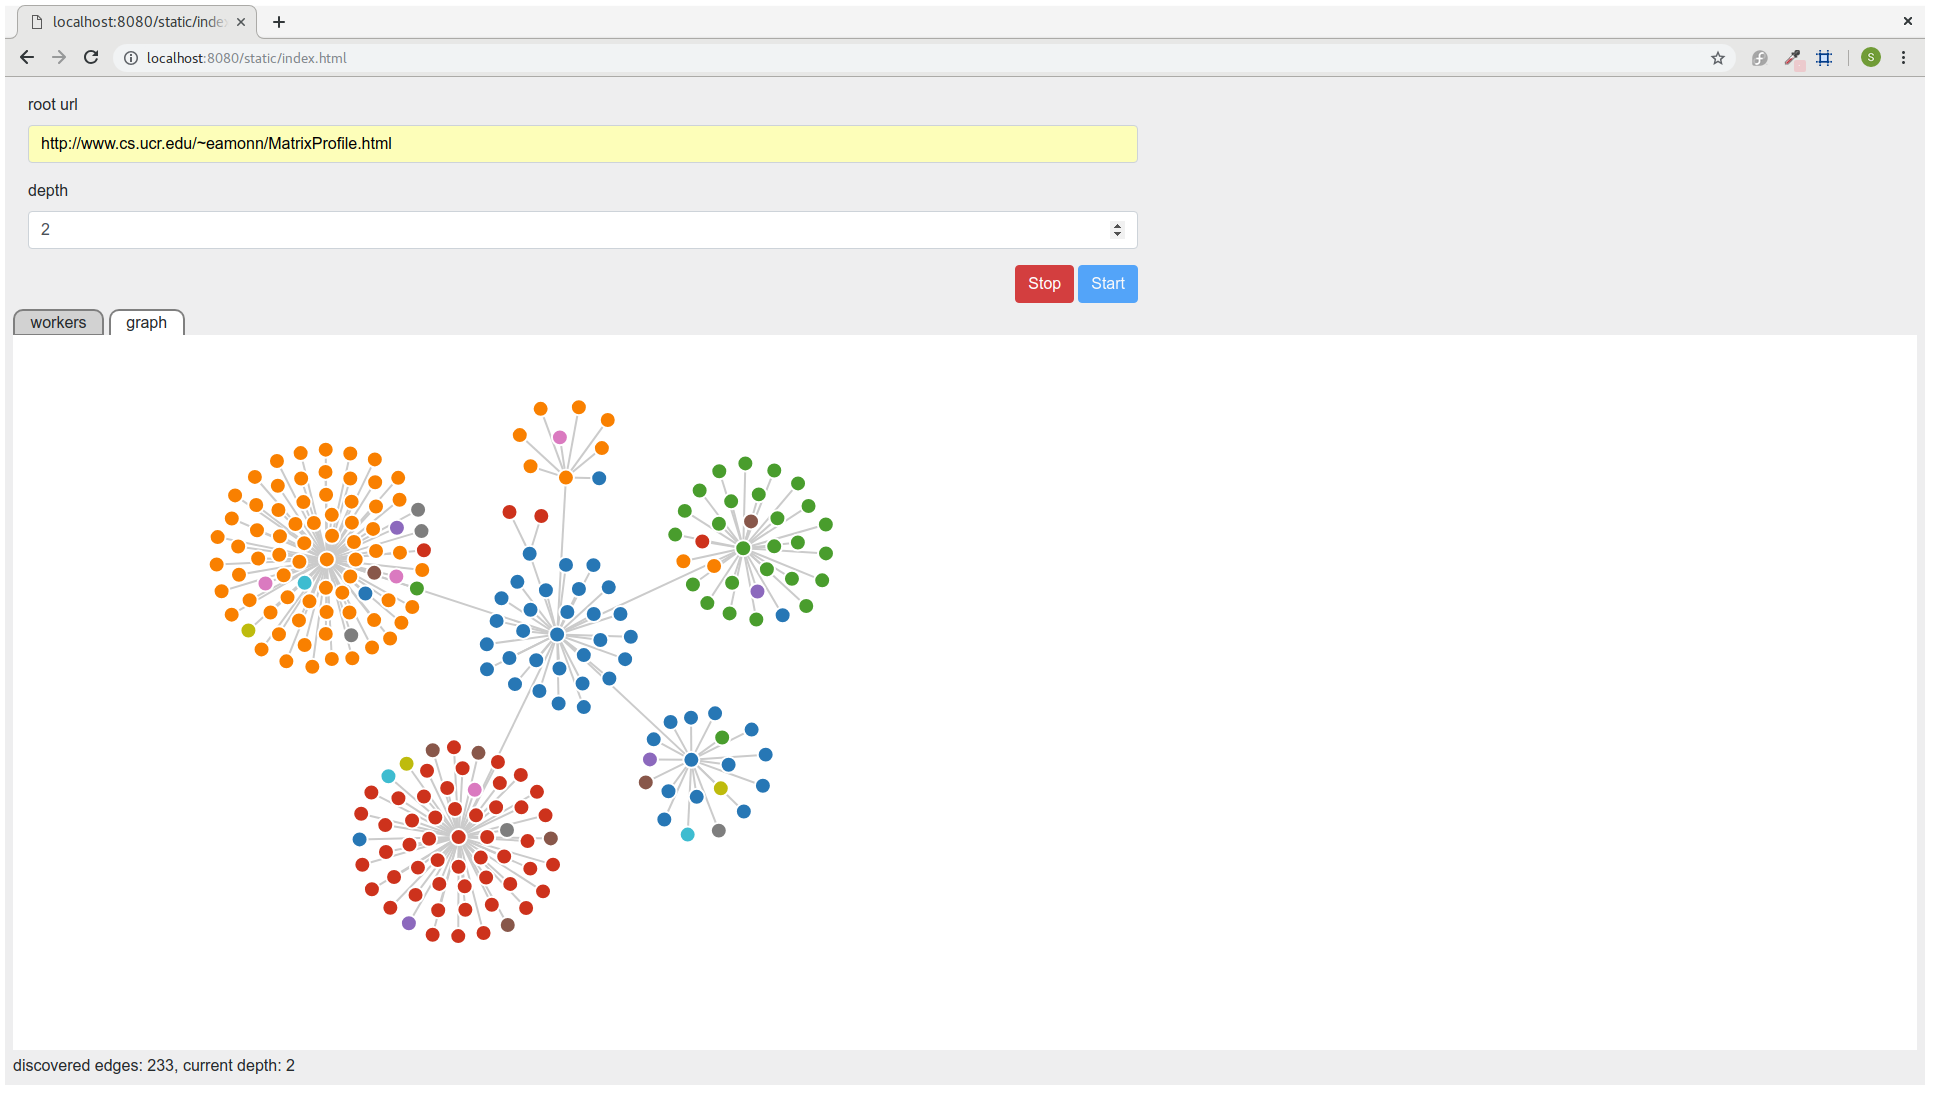
\includegraphics[width=\textwidth]{img/screenshot}
    \caption{Screenshot of the graph view}
    \label{fig:screenshot}
\end{figure}

\subsection{Backend}

\subsubsection{Master}

The master runs a lightweight web server (using
\href{https://bottlepy.org/docs/dev/}{Bottle}, a micro WSGI web framework)
serving the frontend and offers a small REST API for querying the state of the
crawl. This basically consists of starting the crawl and querying the workers
and discovered edges.

The master can be deployed to an EC2 instance using ElasticBeanstalk or run
locally.

\subsubsection{Worker}

The workers are realized as AWS Lambda functions. Lambdas lend themselves naturally
to this task---processing an event (i.e., a new URL which was discovered) is short
and need not store any state except for storing the result. Events are distributed
using a message queue, which is the trigger for the function.

Doing this, we let AWS Lambda take the wheel completely---we do not need to worry
about any aspect of execution and will only be billed what is truly needed, which
would be very hard to gauge for ourselves.

Out of the box, AWS allows 1,000 lambdas be running in parallel. It is possible to increase this number, however, additional procedures are necessary. The time spent waiting for IO operation is critical to this application. Non-blocking IO can further improve the parallelisms of the system and decreasing the cost since a lambda function don't need to sit idle waiting to HTTP responses.

\subsubsection{Storage}

The storage is realized with DynamoDB which is built for handling large amounts of reads and writes up to millions per second.
As the amount of writes scale exponentially with the crawler, it has to have the ability to scale accordingly which DynamoDB provides.
It works with a key:value store, is document driven and fully managed.
The data we need to store is quite simple as it is at most a JSON object with three attributes stored in DynamoDB as a String.
The attributes are the source link, the link found on the website of the source link and the depth or layer of the crawl.
The implementation of the database consists of all function calls to write files to the database, check if an item is in the database and
retrieve both a single item as well as all items in a table. These building blocks allow the master to retrieve data about all the edges
required to draw the graph and it allows the workers to check if the retrieved url is already in the database and if not to write it to the
database together with its source link and the depth of the crawl.

\section{Setup}

We have included setup scripts in \texttt{setup}. They create all resources
used and also set up the needed policies. % make it so this sentence is true

\subsection{Master}

You can either run the master locally using the \texttt{master.py} contained
in the project root. It serves on port 8080.

If you want to deploy it via ElasticBeanstalk, do the following at project
root:

\begin{verbatim}
$ cd eb_master
$ make
\end{verbatim}

The Makefile copies the files properly, runs the EB CLI commands to get
everything ready, attaches the needed policies to your user and also the EC2
instance role which will run the application, and then launches the application
in your default browser. We presume that the AWS and EB CLI are installed and
set up properly.

Once the master is up and running, you can deploy the worker as described in
the next section. The ordering between master and worker is not actually
important.

To terminate the EC2 instance and clean up the files run \texttt{make clean}
later. Please be aware that deletion will take a bit to take effect. Also, the
output tells you that it is fine to Ctrl+C, but don't---while interrupting the
EB CLI (who produces the output) is fine, interrupting \texttt{make} is not.

\subsection{Worker(s)}

The setup and the deployment of the web crawler lambda function have few steps. The directory \texttt{aws\_scripts} stores the scripts used here. The first two steps are the setup of the infrastructure that used by the lambda (queues and DynamoDB). The role lambda-worker-role has the policies to grant the necessary permissions to use these resources. The \texttt{lambda\_worker.py} stores the actual function. The python code and the libraries not provided by the runtime environment are packaged in a ZIP file to be deployed in the AWS, see \texttt{make\_lambda.sh} to further details. The last two steps are the creation of the lambda function QueueInConsumer and mapping one of the queues to it. The script \texttt{create\_all.sh} wraps all the steps described here.

\subsection{Storage}
The setup of the DynamoDB requires permissions of the user and the creation of the tables.
Both are provided as scripts as part of the automation in the build process and are included in the Makefile.

\section{Cost Analysis}

The following analysis considers that we have ten lambdas running in parallel and the throughput of ten URLs per second per lambda. These translate to about 260 millions of URLs per month (10*10*3600*24*365/12) if the system runs at peak efficiency.


\begin{itemize}
    \item The lambda instances consuming less than 128MB of RAM cost US\$ 55 per month (US\$ 0.00000208 per second per instance).
    \item We need to hit the database at least two times per URL; one read to check if it is new, and one write the page. Provisioning the DynamoDB throughput of 100 reads and writes per second with item size of 1 KB is about US\$ 40.
    \item Considering that each page takes 1KB, the storage cost is about US\$ 65.
    \item The standard queue costs US\$0.00000040 per request, therefore, US\$ 105 per month. , for issuing HTTP requests,
\end{itemize}

This estimation is far from comprehensive. However, it gives a lower bound of US\$ 1 per million of URLs to gather them.

\section{Performance}

CloudWatch is the dedicated Monitoring tool of AWS and offers a wide variety of configuration options to display different charts and correlate data.
It offers intersting insights into the performance of the DynamoDB and the Worker Lambdas. The key metrics for a crawl are the Duration of the Lambdas
and the Latency of Reads and Writes for DynamodB as well as the number of Lambdas invoked at any given time.

\begin{figure}[ht]
    \centering
    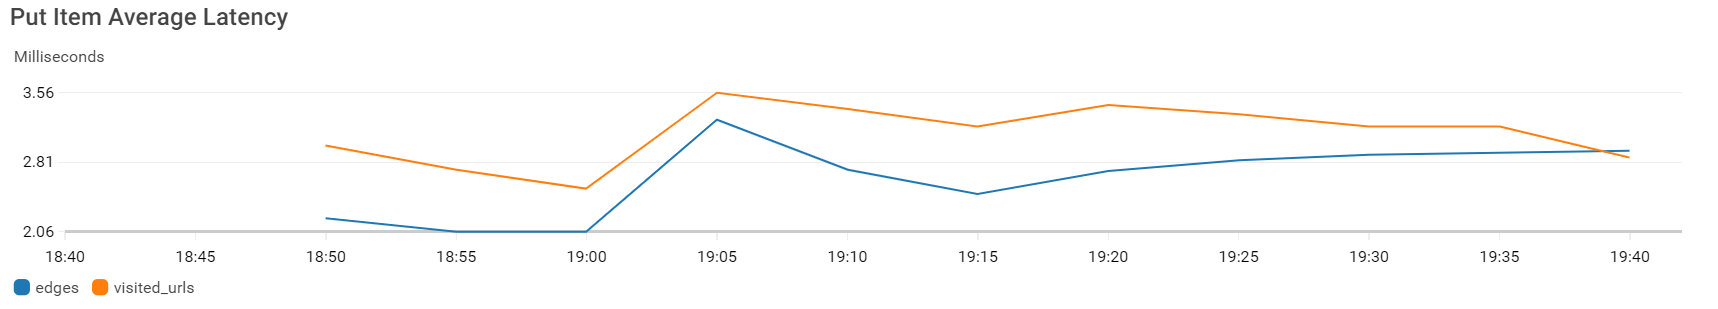
\includegraphics[width=\textwidth]{img/CloudWatchDynamoDBPutItemAverageLatency}
    \caption{Average Latency in ms for an Item to be put into DynamoDB}
    \label{fig:screenshot}
\end{figure}

\begin{figure}
    \centering
    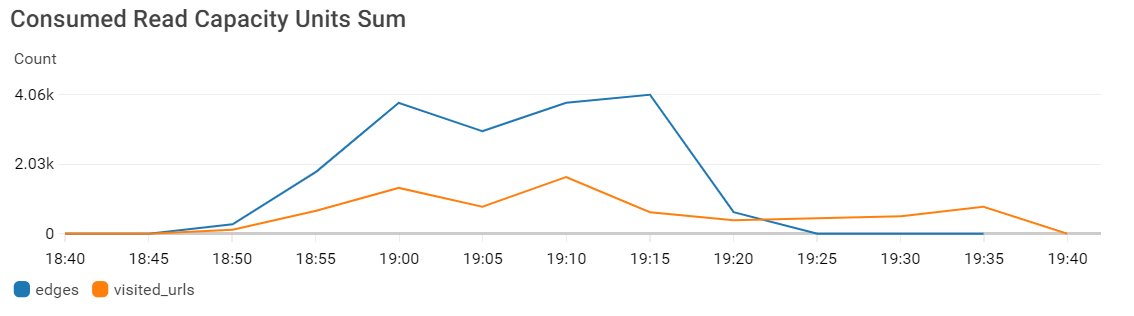
\includegraphics[width=\textwidth]{img/CloudWatchDynamoDBReadCapacityUnitsSum}
    \caption{Number of Reads from DynamoDB}
    \label{fig:screenshot}
\end{figure}

\begin{figure}
    \centering
    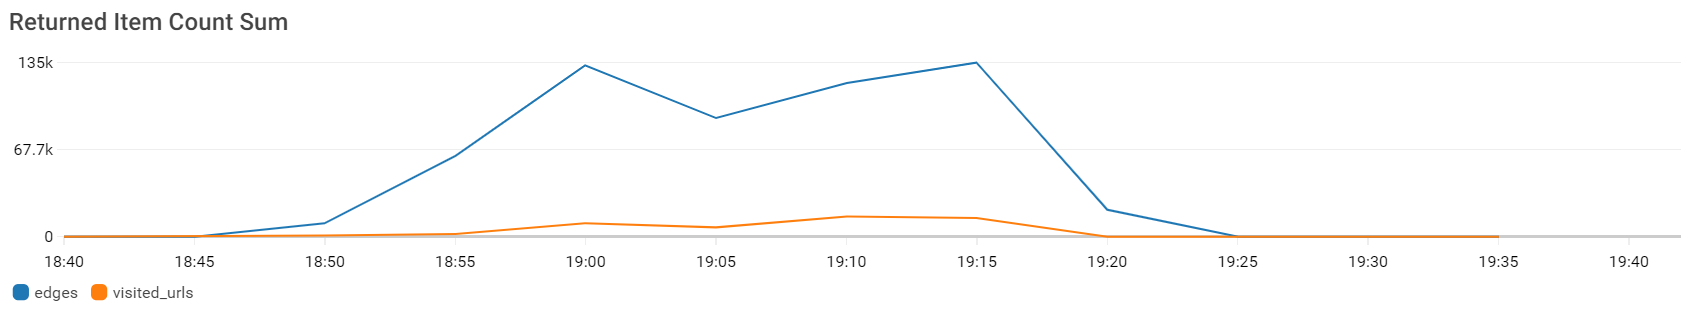
\includegraphics[width=\textwidth]{img/CloudWatchDynamoDBReturnedItemCountSum}
    \caption{Number of Items returned from DynamoDB}
    \label{fig:screenshot}
\end{figure}

\begin{figure}
    \centering
    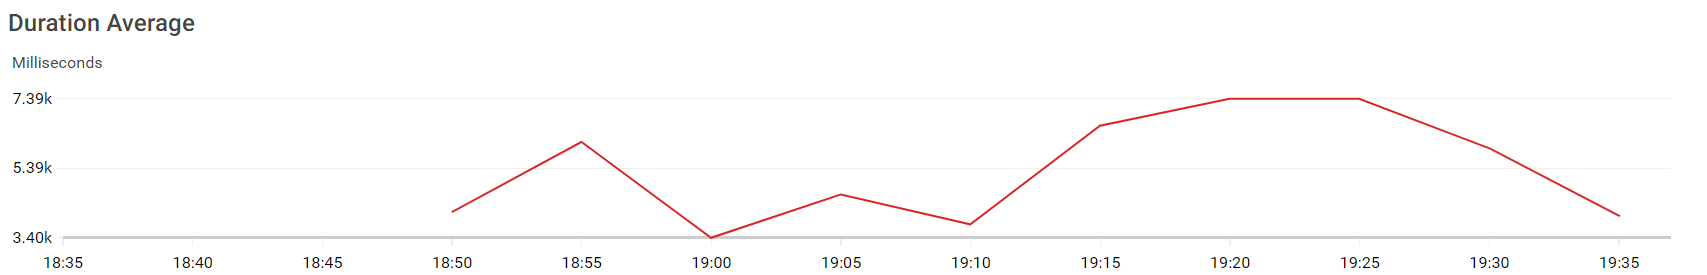
\includegraphics[width=\textwidth]{img/CloudWatchLambdaDurationAverage}
    \caption{Average Duration of the Worker Lambda}
    \label{fig:screenshot}
\end{figure}

\begin{figure}
    \centering
    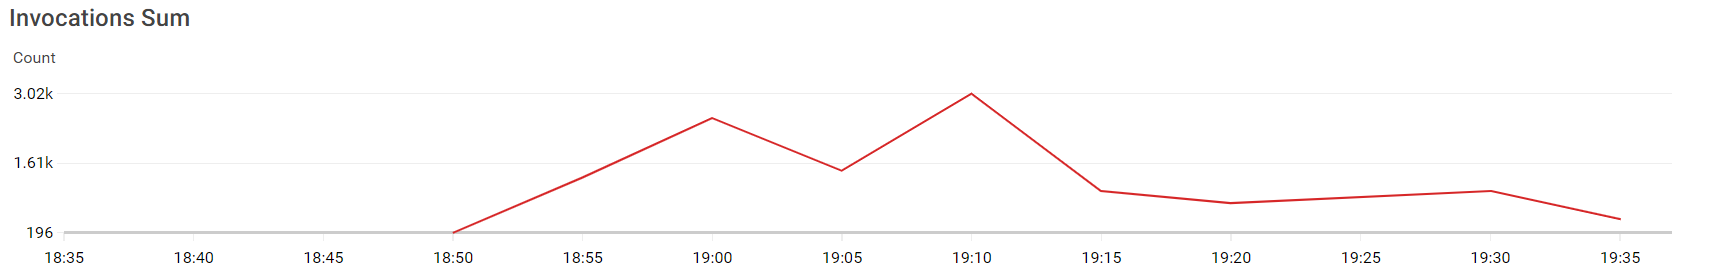
\includegraphics[width=\textwidth]{img/CloudWatchLambdaInvocationsSum}
    \caption{Sum of Invocations of the Worker Lambda}
    \label{fig:screenshot}
\end{figure}


\end{document}
